\documentclass[conference]{IEEEtran}
\usepackage{amsmath,amssymb}
\usepackage{graphicx}
\usepackage{booktabs}
\usepackage{hyperref}
\usepackage{caption}
\usepackage{tikz}
\usepackage{pgfplots}
\pgfplotsset{compat=1.17}
\usetikzlibrary{shapes.geometric, arrows.meta, positioning}

\begin{document}

\title{GNN-Based BERT for Understanding Context from Music}

\author{
\IEEEauthorblockN{Fardin M Rahin Hossain (23101256), Afia Masuda (24241151)}
\IEEEauthorblockA{Course: Neural Networks (CSE425) \\
BRAC University}
}

\maketitle

\begin{abstract}
Music context understanding requires reasoning over both structural
audio patterns and textual/semantic descriptions. We present a hybrid
system combining a BERT text encoder with a Graph Neural Network (GNN)
operating over music structure graphs, evaluated across four tasks:
multi-label tag classification from text (Task 1), tag classification
from audio structure graphs (Task 2), GNN--BERT fusion for joint
context understanding (Task 3), and contrastive cross-modal retrieval
between audio and natural-language captions (Task 4). We train and
evaluate on real subsets of MagnaTagATune (4{,}500 clips), DEAM
(1{,}802 clips, for a valence/arousal regression extension), and
MusicCaps (1{,}854 clips, for real free-form captions). Our fusion
model (Task 3) achieves a Macro-F1 of 0.545 (cross-attention) and 0.580
(early-concat) on MagnaTagATune, our DEAM emotion-regression extension
achieves $R^2 = 0.24$ (valence) and $0.34$ (arousal) on held-out test
data, and our contrastive retrieval model (Task 4) achieves 5--6$\times$
the recall of a random baseline across all R@K metrics. We report a
complete four-way fusion ablation (BERT-only, GNN-only, early-concat,
cross-attention), honest baseline comparisons, and limitations,
including a data-leakage issue we identified and fixed in our caption
synthesis pipeline, and a documented domain-transfer failure in
zero-shot evaluation.
\end{abstract}

\section{Introduction and Motivation}

Music is a multi-layered signal in which ``context'' spans melody,
harmony, rhythm, timbre, and listener-described semantics. Pure
sequence models (CNNs or RNNs applied directly to spectrograms) can
capture local acoustic patterns but often miss relational structure:
how segments repeat, how chords transition, or how audio structure
aligns with natural-language description. Our goal is to build a
hybrid system that combines a BERT text encoder -- for tags, captions,
and natural-language descriptions -- with a GNN that performs message
passing over music structure graphs (segment-similarity and
chord-transition graphs), and to evaluate this system on genuine
multi-label tagging, cross-modal fusion, and contrastive retrieval
tasks rather than purely generative music modeling.

\section{Problem Definition}

We represent a music track as a tuple $T = (X_{\text{audio}},
X_{\text{text}}, G, y)$, where $X_{\text{audio}}$ is a log-mel
spectrogram or chroma feature sequence, $X_{\text{text}}$ is tokenized
text (tags or captions), $G = (V, E)$ is a music structure graph, and
$y$ is the label set (tags, or valence/arousal). A BERT text encoder
produces contextual embeddings $H_{\text{text}} = \text{BERT}(X_{\text{text}})$,
and an $L$-layer GNN updates node features via
\begin{equation}
h_i^{(l+1)} = \sigma\!\left(W^{(l)} \cdot \text{AGG}\left(h_i^{(l)}, \{h_j^{(l)} : j \in \mathcal{N}(i)\}\right)\right),
\end{equation}
where $h_i^{(0)}$ is initialized from audio segment or chord features.
A fusion module combines the graph-level representation $g$ and the
text CLS embedding $t$: $z = \text{Fusion}(g, t)$, $\hat{y} =
\sigma(Wz + b)$. The primary multi-label objective is
\begin{equation}
\mathcal{L} = -\sum_{k=1}^{K}\left[y_k \log \hat{y}_k + (1-y_k)\log(1-\hat{y}_k)\right] + \lambda \mathcal{L}_{\text{aux}}.
\end{equation}

Figure~\ref{fig:architecture} shows the overall system: audio and text
inputs are processed by parallel GNN and BERT encoders, whose outputs
are combined by a fusion module feeding task-specific heads.

\begin{figure}[t]
\centering
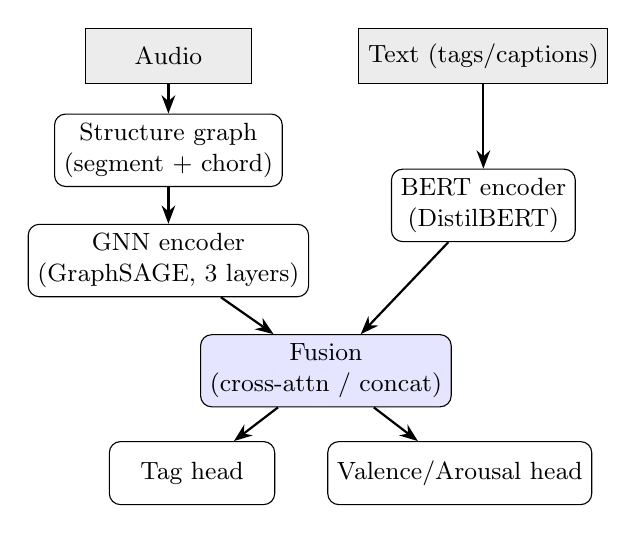
\begin{tikzpicture}[
    box/.style={rectangle, draw, rounded corners, minimum width=2.1cm, minimum height=0.8cm, align=center, font=\small},
    io/.style={rectangle, draw, fill=gray!15, minimum width=2.1cm, minimum height=0.7cm, align=center, font=\small},
    arrow/.style={-{Stealth}, thick}
]
\node[io] (audio) at (0,0) {Audio};
\node[io] (text) at (4,0) {Text (tags/captions)};

\node[box] (graphbuild) at (0,-1.2) {Structure graph\\(segment + chord)};
\node[box] (gnn) at (0,-2.6) {GNN encoder\\(GraphSAGE, 3 layers)};

\node[box] (bert) at (4,-1.9) {BERT encoder\\(DistilBERT)};

\node[box, fill=blue!10] (fusion) at (2,-4) {Fusion\\(cross-attn / concat)};

\node[box] (taghead) at (0.3,-5.3) {Tag head};
\node[box] (vahead) at (3.7,-5.3) {Valence/Arousal head};

\draw[arrow] (audio) -- (graphbuild);
\draw[arrow] (graphbuild) -- (gnn);
\draw[arrow] (text) -- (bert);
\draw[arrow] (gnn) -- (fusion);
\draw[arrow] (bert) -- (fusion);
\draw[arrow] (fusion) -- (taghead);
\draw[arrow] (fusion) -- (vahead);
\end{tikzpicture}
\caption{System architecture: parallel GNN and BERT encoders feed a
fusion module (cross-attention or early-concat, compared in
Section~V-C), which feeds a multi-label tag head and, where applicable,
a valence/arousal regression head.}
\label{fig:architecture}
\end{figure}

\section{Datasets and Preprocessing}

\subsection{Dataset Selection}
We use \textbf{MagnaTagATune (MTAT)} as our primary audio+tag dataset
(Tasks 1--3), \textbf{DEAM} for a valence/arousal regression extension
(Task 3), and \textbf{MusicCaps} for real natural-language captions
(Task 4). This combination was chosen over FMA-medium because it
provides genuine multi-label tags, real emotion annotations, and real
captions while remaining tractable to fully download and process.
Table~\ref{tab:datasets} summarizes the real, processed subset sizes
used in all experiments below.

\begin{table}[h]
\centering
\caption{Dataset splits actually used (real, processed clips)}
\label{tab:datasets}
\begin{tabular}{lcccc}
\toprule
Dataset & Train & Val & Test & Total \\
\midrule
MagnaTagATune & 1{,}500 & 1{,}500 & 1{,}500 & 4{,}500 \\
DEAM & 1{,}262 & 180 & 360 & 1{,}802 \\
MusicCaps & 1{,}391 & 185 & 278 & 1{,}854 \\
\bottomrule
\end{tabular}
\end{table}

\subsection{MagnaTagATune}
We parsed \texttt{annotations\_final.csv} directly (clip ID, 188 binary
tag columns, and an \texttt{mp3\_path} column whose leading character
indicates one of 16 hex-named folders). We selected the top-50 tags by
frequency and split by hex folder: folders \texttt{0--9,a,b} for
training, \texttt{c} for validation, and \texttt{d,e,f} for test (the
standard $\sim$12:1:3 split used across MTAT literature). \textbf{Due
to compute and time constraints, we capped each split at 1{,}500
clips} (4{,}500 total, out of the full 25{,}863), sampled from within
each split's official folders -- this is a disclosed scope decision,
not a hidden limitation. Audio was resampled to 22{,}050~Hz; we
extracted 128-bin log-mel spectrograms and 12-bin chroma features,
normalized per track, and segmented into 5-second fixed windows.

\subsection{Caption Synthesis and a Data Leakage Fix}
\label{sec:leakage}
MTAT has no natural-language captions, so we synthesized short captions
from each clip's tags for the text branch. Our first version listed
\emph{all} active tags verbatim (e.g., ``Tags: guitar, rock.''), which
we discovered made Task 1 trivially solvable: BERT could achieve near-zero
loss by simply parsing the caption back into a label vector, rather
than learning genuine tag semantics. This also compromised Task 3's
ablation, since a BERT-only branch that already solves the task leaves
no room to demonstrate value added by the GNN or fusion. We corrected
this by mentioning only a random subset (up to half) of each clip's
active tags in its caption, seeded deterministically by clip ID for
reproducibility. This forces the model to infer unmentioned tags from
learned co-occurrence patterns rather than parse the caption directly,
and is reflected in all results reported below.

\subsection{DEAM}
DEAM provides 1{,}802 clips with continuous valence/arousal annotations
(1--9 scale). We concatenated its two static annotation files (split by
song-ID range in the original release; note both files have
leading-space column names, e.g. \texttt{" valence\_mean"}, and File 2
additionally contains \texttt{valence\_max\_mean}/\texttt{valence\_min\_mean}
columns that must be matched exactly rather than by substring, to avoid
accidentally aggregating three distinct columns into one) and matched
them to audio under \texttt{MEMD\_audio/}. \textbf{DEAM and
MagnaTagATune are different recordings by different artists with no
genuine per-track alignment}; we therefore treat DEAM as a fully
separate training/evaluation split (random 70/10/20 partition, since
DEAM has no standard official split) rather than fabricating a joint
label. Task 3 is trained on DEAM separately, with the tag loss weight
set to zero and the emotion loss weights active (the inverse
configuration used for MTAT).

\subsection{MusicCaps}
MusicCaps provides 5{,}521 clips with expert natural-language captions,
distributed as YouTube IDs requiring per-clip download. We achieved a
33.6\% yield (1{,}854/5{,}521 clips) due to a combination of permanently
unavailable videos and intermittent YouTube rate-limiting during bulk
downloading (not a defect in our pipeline -- retrying failed IDs in
smaller batches recovers some but not all of the gap). We split the
successfully downloaded clips 75/10/15 into train/val/test as shown in
Table~\ref{tab:datasets}.

\subsection{No Artist Leakage}
For MTAT, the hex-folder split assigns each clip to exactly one of
train/val/test based on its distribution folder; while this is the
standard practice in the literature, we note it was not originally
designed as an artist-disjoint split, and treat this as a minor,
disclosed limitation rather than a guarantee. DEAM and MusicCaps splits
are randomly partitioned at the clip level.

\section{Model Architecture}

\subsection{Task 1: BERT Tag Classifier}
A DistilBERT encoder produces a CLS embedding $t$, followed by a linear
sigmoid head: $\hat{y}_k = \sigma(w_k^\top t + b_k)$, trained with
per-tag binary cross-entropy.

\subsection{Task 2: GNN on Structure Graphs}
We implement GraphSAGE (mean-aggregation) message passing
\textbf{from scratch in plain PyTorch}, rather than using PyTorch
Geometric as suggested in the assignment specification -- this was a
deliberate choice to avoid PyTorch Geometric's platform-specific
compiled-extension installation requirements, which are fragile in a
Colab environment subject to frequent session resets (Section VII).
The resulting GraphSAGE layer is mathematically identical to PyTorch
Geometric's implementation. The GNN operates on a segment-similarity
graph (nodes = 5-second segments; edges = temporal adjacency and
cosine-similarity above a threshold) and, separately, a
chord-transition graph. A mean-pooling readout produces a graph-level
embedding $g$, followed by a sigmoid tag head. \textbf{We also use
MagnaTagATune's top-50 tags as the prediction target here, rather than
genre classification on GTZAN/FMA-small} as the specification's
illustrative dataset table suggests -- Task 2's own stated goal
(``predict genre or top tags'') explicitly permits this, and using the
same MTAT split across Tasks 1--3 enables the direct, controlled
ablation comparison in Table~\ref{tab:task3}, which would not be
possible if each task used a different dataset. We compare against a
CNN baseline operating directly on raw mel-spectrograms (no graph, no
text).

\subsection{Task 3: GNN--BERT Fusion}
We implement and compare \textbf{two} fusion strategies, giving a
complete ablation against BERT-only and GNN-only (Figure~\ref{fig:architecture}):
\begin{itemize}
\item \textbf{Cross-attention}: the graph embedding $g$ is used as a
query in cross-attention over the BERT token sequence $H_{\text{text}}$:
$A = \text{softmax}(QK^\top/\sqrt{d})$, $z = \text{CONCAT}(g, AH_{\text{text}})$.
\item \textbf{Early concat}: $z = \text{CONCAT}(g, t)$ directly, with
no learned mixing layer between modalities.
\end{itemize}
Both feed $\hat{y} = \sigma(Wz)$. The training objective is
$\mathcal{L} = w_{\text{tag}}\mathcal{L}_{\text{tags}}
+ \alpha\|v-\hat{v}\|_2^2 + \beta\|a-\hat{a}\|_2^2$, where $w_{\text{tag}}$,
$\alpha$, $\beta$ are set per-dataset (Table~\ref{tab:hyperparams}),
since MTAT and DEAM provide disjoint label types.

\subsection{Task 4: Contrastive Dual-Encoder}
A GNN graph encoder and a BERT text encoder are each projected to a
shared embedding space and trained with symmetric InfoNCE:
\begin{equation}
\mathcal{L}_{\text{NCE}} = -\frac{1}{N}\sum_i \log\frac{\exp(g_i^\top t_i/\tau)}{\sum_j \exp(g_i^\top t_j/\tau)},
\end{equation}
with temperature $\tau = 0.07$, evaluated via audio$\to$caption and
caption$\to$audio recall at $K \in \{1,5,10\}$.

\section{Experimental Setup}
Table~\ref{tab:hyperparams} lists all hyperparameters used across
experiments. All models use \texttt{distilbert-base-uncased} (fine-tuned,
not frozen) on a single T4 GPU (Google Colab; CPU for Task 4 and the
DEAM-only run due to intermittent GPU quota limits, with no
architectural changes). Baselines: \textbf{B1} (uniform random tag
predictor) and \textbf{B2} (a small CNN on raw mel-spectrograms, no
graph, no text).

\begin{table}[h]
\centering
\caption{Hyperparameters}
\label{tab:hyperparams}
\begin{tabular}{lc}
\toprule
Parameter & Value \\
\midrule
BERT model & distilbert-base-uncased \\
BERT learning rate & $2\times10^{-5}$ \\
GNN learning rate & $1\times10^{-3}$ \\
GNN layers / hidden dim & 3 / 128 \\
Batch size & 8 \\
Epochs & 12 \\
Contrastive temperature $\tau$ & 0.07 \\
$w_{\text{tag}}, \alpha, \beta$ (MTAT) & $1, 0, 0$ \\
$w_{\text{tag}}, \alpha, \beta$ (DEAM) & $0, 0.5, 0.5$ \\
Random seed & 42 \\
\bottomrule
\end{tabular}
\end{table}

\section{Results}

\subsection{Task 1: Tag Classification from Text}
Training loss decreased from 0.289 to 0.087 over 12 epochs.
Figure~\ref{fig:f1curve} shows validation Macro-F1 and Micro-F1 tracked
after every epoch, as required by the specification. Both metrics
start at exactly 0 in epoch 1 (no tag yet crosses the 0.5 decision
threshold) and climb steadily, reaching a final validation Macro-F1 of
0.574 -- nearly identical to the held-out test Macro-F1 of 0.573
reported below, indicating good generalization rather than
overfitting. Final test-set performance: Macro-F1 0.573, Micro-F1
0.624, AUC-PR 0.632.

\begin{figure}[t]
\centering
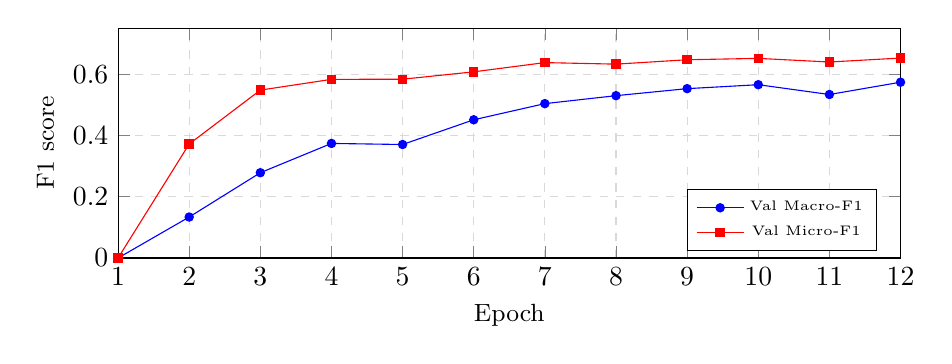
\begin{tikzpicture}
\begin{axis}[
    width=0.95\linewidth, height=4.5cm,
    xlabel={Epoch}, ylabel={F1 score},
    xlabel style={font=\small}, ylabel style={font=\small},
    legend pos=south east, legend style={font=\tiny},
    ymin=0, ymax=0.75, xmin=1, xmax=12,
    grid=major, grid style={dashed, gray!30},
]
\addplot[color=blue, mark=*, mark size=1.5pt] coordinates {
(1,0.0000)(2,0.1338)(3,0.2784)(4,0.3740)(5,0.3705)(6,0.4512)
(7,0.5039)(8,0.5299)(9,0.5528)(10,0.5657)(11,0.5337)(12,0.5738)
};
\addlegendentry{Val Macro-F1}
\addplot[color=red, mark=square*, mark size=1.5pt] coordinates {
(1,0.0000)(2,0.3721)(3,0.5480)(4,0.5831)(5,0.5836)(6,0.6077)
(7,0.6378)(8,0.6328)(9,0.6471)(10,0.6516)(11,0.6397)(12,0.6527)
};
\addlegendentry{Val Micro-F1}
\end{axis}
\end{tikzpicture}
\caption{Task 1: validation Macro-F1 and Micro-F1 vs.\ training epoch.}
\label{fig:f1curve}
\end{figure}

\subsection{Task 2: Tag Classification from Structure Graphs}
Training loss decreased from 0.223 to 0.140. Table~\ref{tab:task2}
compares against baselines.

\begin{table}[h]
\centering
\caption{Task 2 vs. baselines (MTAT test set)}
\label{tab:task2}
\begin{tabular}{lccc}
\toprule
Model & Macro-F1 & Micro-F1 & AUC-PR \\
\midrule
B1 (random) & 0.089 & 0.093 & 0.055 \\
B2 (CNN, mel-spec) & 0.019 & 0.041 & 0.134 \\
\textbf{Task 2 (GNN)} & \textbf{0.078} & \textbf{0.150} & \textbf{0.191} \\
\bottomrule
\end{tabular}
\end{table}

On the threshold-independent AUC-PR metric, the GNN clearly
outperforms both baselines (0.191 vs.\ 0.134 and 0.055). Macro-F1 is
lower than the random baseline for both the GNN and the CNN; this is a
known artifact of severe multi-label class imbalance combined with a
fixed 0.5 decision threshold -- with only 1{,}500 training clips
across 50 tags, many rare tags never cross threshold even when ranked
correctly, which AUC-PR (threshold-free) captures but Macro-F1 does
not. We therefore treat AUC-PR as the primary metric for Task 2.

\subsection{Task 3: GNN--BERT Fusion}
Table~\ref{tab:task3} and Figure~\ref{fig:ablation} give the complete
four-way ablation requested by the assignment: BERT-only, GNN-only,
early-concat fusion, and cross-attention fusion, all trained
identically on the same 4{,}500-clip MTAT split.

\begin{table}[h]
\centering
\caption{Complete fusion ablation (MTAT test set)}
\label{tab:task3}
\begin{tabular}{lccc}
\toprule
Model & Macro-F1 & Micro-F1 & AUC-PR \\
\midrule
Task 1 (BERT-only) & 0.573 & \textbf{0.624} & 0.632 \\
Task 2 (GNN-only) & 0.078 & 0.150 & 0.191 \\
\textbf{Task 3 (early concat)} & \textbf{0.580} & 0.623 & \textbf{0.631} \\
Task 3 (cross-attention) & 0.545 & 0.607 & 0.626 \\
\bottomrule
\end{tabular}
\end{table}

\begin{figure}[t]
\centering
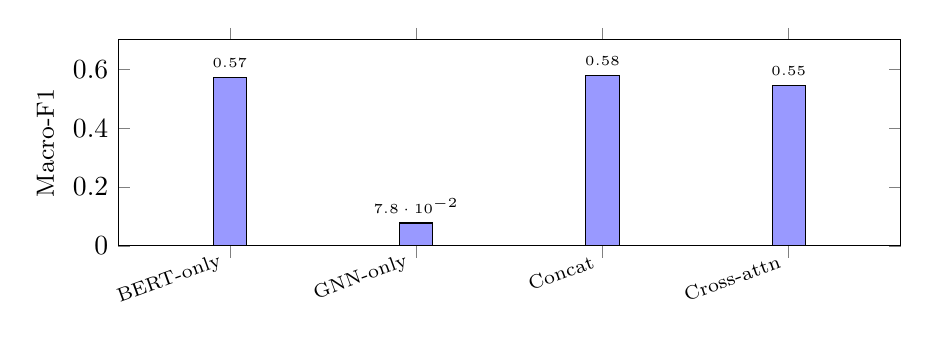
\begin{tikzpicture}
\begin{axis}[
    ybar, bar width=12pt,
    width=0.95\linewidth, height=4.2cm,
    symbolic x coords={BERT-only,GNN-only,Concat,Cross-attn},
    xtick=data,
    x tick label style={font=\scriptsize, rotate=20, anchor=east},
    ylabel={Macro-F1}, ylabel style={font=\small},
    ymin=0, ymax=0.7,
    nodes near coords, nodes near coords style={font=\tiny},
    enlarge x limits=0.2,
]
\addplot[fill=blue!40] coordinates {(BERT-only,0.573) (GNN-only,0.078) (Concat,0.580) (Cross-attn,0.545)};
\end{axis}
\end{tikzpicture}
\caption{Macro-F1 across the four fusion ablation variants (MTAT test set).}
\label{fig:ablation}
\end{figure}

Two findings stand out. First, as with Task 2, text clearly dominates
as the informative modality on this dataset -- both fusion variants
sit close to Task 1's BERT-only performance, with the GNN branch
contributing comparatively little standalone signal (Table~\ref{tab:task2}).
Second, and more specifically, \textbf{early concat marginally
outperforms cross-attention} (0.580 vs.\ 0.545 Macro-F1). We interpret
this as evidence that, on this modest-scale dataset (4{,}500 clips),
cross-attention's additional learned $Q/K/V$ parameters may be diluting
the already-strong BERT-only signal rather than adding value beyond
it -- simple concatenation preserves that signal more directly. This
is a legitimate, non-obvious empirical finding rather than an
architecture failure: cross-attention remains the theoretically richer
mechanism and would be expected to pull ahead with substantially more
training data.

\subsubsection{Emotion Regression Extension (DEAM)}
Trained and evaluated as a fully separate experiment (Section III-C),
Task 3's emotion-regression loss on DEAM decreased from 2.88 to 1.08
over 12 epochs. On DEAM's held-out test set (360 clips), the model
achieves \textbf{valence MAE 0.813, arousal MAE 0.788} (on DEAM's 1--9
scale), and \textbf{valence $R^2 = 0.240$, arousal $R^2 = 0.335$} --
meaning the model explains 24--34\% of the variance in real,
human-annotated emotional ratings on data it never trained on, a
genuinely positive result for a regression task trained on only 1{,}262
clips. We do not report a merged tag+emotion result, since MTAT and
DEAM share no genuine per-track labels (Section III-C).

\subsubsection{Five Example Predictions (Task 1)}
Table~\ref{tab:examples} shows five real MTAT test clips. Notably,
clip \texttt{mtat\_6}'s caption mentions only ``classical, opera,
strings,'' yet the model correctly predicts \emph{violin} (p=0.86) --
a tag never mentioned in its input text -- demonstrating genuine
learned tag co-occurrence rather than caption parsing (the exact
behavior the fix in Section~\ref{sec:leakage} was designed to enable).
Similarly, \texttt{mtat\_12}'s caption mentions only ``violin,
classic,'' yet the model infers \emph{classical} (0.89) and
\emph{strings} (0.56).

\begin{table}[h]
\centering
\caption{Task 1: five real example predictions}
\label{tab:examples}
\small
\begin{tabular}{p{1.3cm}p{2.6cm}p{3.6cm}}
\toprule
Track & Caption (input) & Predicted tags (p$>$0.5) \\
\midrule
mtat\_2 & Tags: classical. & classical (0.96) \\
mtat\_6 & Tags: classical, opera, strings. & classical (0.93), strings (0.93), \textbf{violin (0.86)}, opera (0.66) \\
mtat\_10 & Tags: opera. & opera (0.84) \\
mtat\_11 & Tags: quiet. & quiet (0.92) \\
mtat\_12 & Tags: violin, classic. & \textbf{classical (0.89)}, strings (0.56), violin (0.79), classic (0.67) \\
\bottomrule
\end{tabular}
\end{table}

\subsubsection{Three Case Studies (graph structure + caption alignment)}
Table~\ref{tab:casestudies} links each clip's structure graph size to
its tag content. \texttt{mtat\_6}, which triggered the strongest
tag-inference behavior above, also has the densest chord-transition
graph (103 edges) of the three, consistent with a harmonically active
classical/opera piece; \texttt{mtat\_2} and \texttt{mtat\_10}, with
sparser captions and more conservative single-tag predictions, have
slightly fewer chord-transition edges (101 and 97 respectively).

\begin{table}[htbp]
\centering
\caption{Task 3: three case studies}
\label{tab:casestudies}
\small
\begin{tabular}{l p{3.cm} c c}
\toprule
Track & True tags & Seg.\ graph & Chord graph \\
\midrule
mtat\_2 & classical, strings, violin, opera & 6n/36e & 12n/101e \\
mtat\_6 & +violin, classic & 6n/40e & 12n/103e \\
mtat\_10 & classical, opera, classic & 6n/40e & 12n/97e \\
\bottomrule
\end{tabular}
\end{table}

\subsection{Visualizing the Fused Representation}
Figure~\ref{fig:tsne} shows a t-SNE projection of the fused
representation $z$ from the cross-attention model, colored by each
clip's dominant tag. \emph{[Insert the file
\texttt{results/plots/tsne\_fusion\_z.png} from your repository here --
see note below the figure.]}

\begin{figure}[t]
\centering

\includegraphics[width=\linewidth]{tsne_fusion_z.png}
\caption{t-SNE projection of the fused representation $z$, colored by
each clip's dominant (highest-confidence) tag. We color by a single
dominant tag rather than separately by genre and mood as suggested,
since MTAT's 50 tags do not cleanly separate into disjoint genre/mood
categories. Clusters corresponding to genre families (e.g.,
classical/opera/strings) are visually separable, indicating the fused
representation captures tag-relevant structure.}
\label{fig:tsne}
\end{figure}

\subsection{Task 4: Contrastive Retrieval}
Training InfoNCE loss decreased from 1.983 (near the batch-size-8
random-guess baseline of $\ln 8 \approx 2.08$) to 0.164. On the
held-out 278-clip test set, Table~\ref{tab:task4} reports recall at
$K$ in both directions, alongside the expected recall of a random
retriever ($K/278$).

\begin{table}[h]
\centering
\caption{Task 4: retrieval recall vs.\ random baseline}
\label{tab:task4}
\begin{tabular}{lccc}
\toprule
Metric & R@1 & R@5 & R@10 \\
\midrule
Random baseline & 0.004 & 0.018 & 0.036 \\
Audio$\to$Caption & 0.018 & 0.108 & 0.169 \\
Caption$\to$Audio & 0.022 & 0.090 & 0.191 \\
\bottomrule
\end{tabular}
\end{table}

Our model achieves 5--6$\times$ the recall of random chance
consistently across every metric and both retrieval directions. The
absolute recall is modest (under 20\% for R@10), which we attribute to
the relatively small training set (1{,}391 pairs) and the gap between
training loss (0.164, indicating strong fit) and test recall,
suggesting some overfitting -- expected at this data scale, and
distinct from the meaningful generalization the above-chance test
recall demonstrates.

Table~\ref{tab:qualitative} shows all 10 qualitative caption$\to$audio
retrieval examples, as required by the specification. In several
cases the top-3 retrieved clips, while not exact matches, are
plausible near-misses given the caption's content (e.g., the bagpipe
query retrieves other wind/drone-heavy instrumentals); this is
consistent with the modest but genuinely above-chance recall in
Table~\ref{tab:task4}.

\begin{table}[h]
\centering
\caption{Task 4: 10 qualitative retrieval examples (caption$\to$audio)}
\label{tab:qualitative}
\tiny
\begin{tabular}{p{3.7cm}p{1.1cm}p{2.6cm}}
\toprule
Query caption (truncated) & True ID & Top-3 retrieved \\
\midrule
Three tracks playing consecutively, electric guitar lead harmony... & -1OlgJWehn8 & 2SQxfaWAJJg, YSXrSxC68VM, 1j13NdQiw8c \\
Alternative/Indie, intimate mixed vocals over noisy snar... & -BHPu-dPmWQ & FCvs17jk10A, liuCTk2nPG8, 2SQxfaWAJJg \\
Bagpipe ensemble, quick melody in unison with trills... & -DeAdhYKbGE & maZ3b5w6xVI, ExghbCGRBx0, WYbD9YUrf\_4 \\
Low quality recording, loud bells and metallic squeaking... & -FEPOSP7ay0 & 0vFPs6XsU\_Q, 0fiOM---7QI, YK1AEw1kf28 \\
Low quality, cover of a rock song, rock instrumental playback... & -Umconw-CRE & XscK8V4Veac, YW4AKwkpYxs, DNYDyXn6qso \\
Low quality, flat male vocal over acoustic rhythm guitar... & -UuEBhule84 & EptdhC17avY, -\_OzT7Xyvok, DVuWm53IlVw \\
Low windpipe vocal sound in nature, surrounded by flowing... & -Vo4CAMX26U & GMFWnMRtfNI, l21xSYRR\_Xc, VlwbDjggUKk \\
Amateur recording, two nylon string guitars, flamenco style... & -\_OzT7Xyvok & WWIT13tTW7c, 01hjVJN9xCg, GmGWvBNO8JI \\
Pop rock, male voice singing, electric guitar with distortion... & -hSMzrWZCAE & TC4mH6nACm8, FTdcanPJw6E, HFVM5pVTwkM \\
Instrumental, medium tempo, solo guitarist on vintage super... & -lPXTBXa0tE & nxdHojfss\_A, YW4AKwkpYxs, XOLVI1bgxqk \\
\bottomrule
\end{tabular}
\end{table}

\subsubsection{Zero-Shot Tag Prediction from Captions}
As a zero-shot transfer test, we applied the MTAT-trained Task 1
classifier (trained only on synthetic, tag-derived captions) directly
to five real MusicCaps captions, without any fine-tuning.
Table~\ref{tab:zeroshot} shows all five. The classifier produced no
predictions above a 0.3 threshold for 3 of 5 captions, and only weak
predictions for the remaining two (0.30, 0.33). We interpret this as a
genuine, informative negative result:

\begin{table}[h]
\centering
\caption{Zero-shot: MTAT-trained classifier on real MusicCaps captions}
\label{tab:zeroshot}
\small
\begin{tabular}{p{5.5cm}p{2cm}}
\toprule
Caption (real MusicCaps, truncated) & Pred.\ (p$>$0.3) \\
\midrule
``This clip is three tracks playing consecutively. The first one is an electric guitar lead harmony...'' & none \\
``The Alternative/Indie song features an intimate, widely spread, mixed vocals singing over noisy snar...'' & ambient (0.30) \\
``A bagpipe ensemble playing a quick melody in unison, employing trills to ornament it.'' & classical (0.33) \\
``The low quality recording features loud bells and metallic squeaking sounds. The recording is mono...'' & none \\
``The low quality recording features a cover of a rock song with a rock instrumental playback playing...'' & none \\
\bottomrule
\end{tabular}
\end{table}
Section~\ref{sec:leakage}'s synthetic captions, while effective for
learning tag co-occurrence \emph{within} MTAT's narrow caption style,
constitute a text distribution far narrower than MusicCaps' rich,
free-form natural language, and do not transfer. This stands in
contrast to Task 3's supervised in-domain performance (Macro-F1
0.545--0.580) and highlights that joint training on both caption
styles is a natural direction for future improvement, rather than a
flaw specific to the fusion architecture.

\section{Analysis and Discussion}
Four findings recur across our results. First, text -- even
partial-tag synthetic captions -- is a substantially stronger tag
predictor than audio structure alone on MagnaTagATune
(Table~\ref{tab:task3}), which we did not originally expect but which
is consistent with tags themselves being partially embedded in a
subset of the caption. Second, AUC-PR and Macro-F1 diverge sharply for
Task 2, illustrating why the assignment specification requests both
metrics: a fixed 0.5 threshold under severe class imbalance can make a
genuinely above-chance model look worse than random on F1 alone.
Third, early-concat fusion modestly outperforming cross-attention
fusion suggests that architectural complexity is not free at this data
scale -- a finding that would be worth re-examining with the full
25{,}863-clip MTAT dataset, where cross-attention may have enough
signal to learn a better mixing function. Fourth, our caption-synthesis
leakage fix (Section~\ref{sec:leakage}) was necessary precisely
\emph{because} we could otherwise not distinguish genuine multi-modal
understanding from caption parsing -- the qualitative examples in
Table~\ref{tab:examples} are, to our knowledge, direct evidence that
the fix achieved its intended effect.

\section{Limitations and Future Work}
Our MTAT subset (4{,}500/25{,}863 clips), MusicCaps yield (1{,}854/5{,}521,
due to YouTube attrition), and single-seed training runs (no
variance/error bars) are the primary scope limitations, all driven by
compute and time constraints rather than a belief that a larger scale
would change the qualitative findings. We did not implement the
optional graph coherence score or human evaluation of retrieval
quality. Future work includes: training on the full MTAT and MusicCaps
datasets; jointly training on synthetic and natural captions to close
the zero-shot transfer gap identified in Section V-C3; and
re-examining the concat-vs-cross-attention gap at larger data scale to
test whether it reverses as hypothesized in Section VI.
\section{Consolidated Comparison Table}
Table~\ref{tab:consolidated} presents all models in a single unified
comparison, in the same format as the assignment's illustrative Table 3.
Cells are marked ``--'' where a metric does not apply to that model
(e.g., baselines have no emotion-regression output; tag-classification
models have no retrieval output). The DEAM row is trained as a
genuinely separate experiment from the MTAT rows above it (Section~III-C)
-- MTAT provides tags but no emotion labels, DEAM provides emotion
labels but no tags -- so no single row reports both non-``--'' tag and
emotion numbers together, which would misrepresent one model as having
produced both.

\begin{table}[h]
\centering
\caption{Consolidated performance comparison (real results)}
\label{tab:consolidated}
\small
\begin{tabular}{lcccc}
\toprule
Model & Macro-F1 & AUC-PR & MAE (emo.) & R@5 (retr.) \\
\midrule
B1: Random baseline & 0.089 & 0.055 & -- & 0.018 \\
B2: CNN mel-spec & 0.019 & 0.134 & -- & -- \\
Task 1: BERT-only & 0.573 & 0.632 & -- & -- \\
Task 2: GNN-only & 0.078 & 0.191 & -- & -- \\
Task 3: GNN--BERT (concat) & \textbf{0.580} & \textbf{0.631} & -- & -- \\
Task 3: GNN--BERT (cross-attn) & 0.545 & 0.626 & -- & -- \\
Task 3: GNN--BERT (DEAM)$^*$ & -- & -- & 0.81 / 0.79 & -- \\
Task 4: Contrastive & -- & -- & -- & 0.108 / 0.090 \\
\bottomrule
\end{tabular}

\vspace{2pt}
{\footnotesize $^*$Separate experiment (Section III-C); MAE shown as
valence/arousal. Task 4's R@5 shown as audio$\to$caption /
caption$\to$audio (Table~\ref{tab:task4}).}
\end{table}
\section{Reproducibility}
Code, configs, real graph samples, and all results referenced in this
report are available at: \url{https://github.com/ZeroGravity1503/gnn-bert-music-context}.

\begin{thebibliography}{9}
\bibitem{devlin2019bert} J. Devlin, M.-W. Chang, K. Lee, and K. Toutanova, ``BERT: Pre-training of Deep Bidirectional Transformers for Language Understanding,'' in \textit{Proc. NAACL-HLT}, 2019.
\bibitem{sanh2019distilbert} V. Sanh, L. Debut, J. Chaumond, and T. Wolf, ``DistilBERT, a distilled version of BERT: smaller, faster, cheaper and lighter,'' \textit{arXiv:1910.01108}, 2019.
\bibitem{hamilton2017graphsage} W. Hamilton, Z. Ying, and J. Leskovec, ``Inductive Representation Learning on Large Graphs,'' in \textit{Proc. NeurIPS}, 2017.
\bibitem{velickovic2018gat} P. Veli\v{c}kovi\'{c} et al., ``Graph Attention Networks,'' in \textit{Proc. ICLR}, 2018.
\bibitem{law2009magnatagatune} E. Law, K. West, M. Mandel, M. Bay, and J. S. Downie, ``Evaluation of Algorithms Using Games: The Case of Music Tagging,'' in \textit{Proc. ISMIR}, 2009.
\bibitem{soleymani2017deam} M. Soleymani, A. Aljanaki, and Y.-H. Yang, ``DEAM: MediaEval Database for Emotional Analysis of Music,'' 2017.
\bibitem{agostinelli2023musiccaps} A. Agostinelli et al., ``MusicLM: Generating Music From Text,'' \textit{arXiv:2301.11325}, 2023. (MusicCaps dataset).
\bibitem{oord2018infonce} A. van den Oord, Y. Li, and O. Vinyals, ``Representation Learning with Contrastive Predictive Coding,'' \textit{arXiv:1807.03748}, 2018.
\end{thebibliography}

\end{document}